\documentclass[../../main.tex]{subfiles}
\begin{document}

\begin{flushright}
\footnotesize\textit{【自動文字起こし・要確認】}
\end{flushright}

{\bf [解]} (1) $r(n) = \dfrac{a}{2^n}$ とおく． $O_n$ を原点とし，$\vec{O_n O_{n+1}}$ を $x$ 軸とする下図のような平面をとる．この平面での $S_n, S_{n+1}$ の断面は
\begin{align}
C_n &: x^2 + y^2 = r(n)^2 \\
C_{n+1} &: (x - r(n))^2 + y^2 = r(n+1)^2
\end{align}
であり，これらの交点の $x$ 座標は，
\begin{align}
x = \dfrac{-r(n+1)^2 + 2r(n)^2}{2r(n)} = \dfrac{7a}{2^{n+3}}
\end{align}
である．ここで，$x, y$ 軸へ $\dfrac{2^n}{a}$ 倍した座標で考えれば，もとめる体積 $V_n$ は
\begin{align}
\Bigl( \dfrac{2^n}{a} \Bigr)^3 V_n &= \pi \int_{\frac{7}{8}}^{\frac{1}{2}} \Bigl\{ \dfrac{1}{4} - (x-1)^2 \Bigr\} dx + \pi \int_{\frac{7}{8}}^1 (1 - x^2) dx \\
&= \pi \int_{\frac{1}{8}}^{\frac{1}{2}} \Bigl( \dfrac{1}{4} - x^2 \Bigr) dx + \pi \int_{\frac{7}{8}}^1 (1 - x^2) dx \quad \cdots \text{①}
\end{align}
各項計算して，
\begin{itemize}
  \item $\displaystyle \int_{\frac{1}{8}}^{\frac{1}{2}} \Bigl(\dfrac{1}{4} - x^2\Bigr) dx = \Bigl[ \dfrac{1}{4} x - \dfrac{1}{3} x^3 \Bigr]_{\frac{1}{8}}^{\frac{1}{2}} = \dfrac{1}{4} \Bigl( \dfrac{1}{2} - \dfrac{1}{8} \Bigr) - \dfrac{1}{3} \Bigl( \dfrac{1}{8} - \dfrac{1}{8^3} \Bigr) = \dfrac{27}{8 \cdot 64}$
  \item $\displaystyle \int_{\frac{7}{8}}^1 (1 - x^2) dx = \Bigl[ x - \dfrac{1}{3} x^3 \Bigr]_{\frac{7}{8}}^1 = \dfrac{2}{3} - \Bigl( \dfrac{7}{8} - \dfrac{1}{3} \Bigl( \dfrac{7}{8} \Bigr)^3 \Bigr) = \dfrac{23}{3 \cdot 8^3}$
\end{itemize}
だから，①より
\begin{align}
V_n &= \pi \Bigl(\dfrac{a}{2^n}\Bigr)^3 \Bigl\{ \dfrac{27}{8^3} + \dfrac{23}{3 \cdot 8^3} \Bigr\} \\
&= \pi \Bigl(\dfrac{a}{2^{n+3}}\Bigr)^3 \cdot \dfrac{104}{3}
\end{align}

\paragraph{(2)}
\begin{align}
V_m &= \dfrac{104 a^3 \pi}{3} \sum_{n=1}^m \Bigl(\dfrac{1}{2^{n+3}}\Bigr)^3 \\
&= \dfrac{104 a^3 \pi}{3} \Bigl(\dfrac{1}{2^4}\Bigr)^3 \dfrac{1 - (1/2)^{3m}}{1 - (1/2)^3} \\
&\xrightarrow{m \to \infty} \dfrac{13}{1344} a^3 \pi
\end{align}

\bigskip\noindent{\bf [解注]}
$V_n$ の求値に球帽公式を用いると，
\begin{itemize}
  \item $\displaystyle \int_{\frac{1}{8}}^{\frac{1}{2}} \Bigl(\dfrac{1}{4} - x^2\Bigr) dx = \dfrac{3/8}{2 \cdot 1/2} \cdot \dfrac{4}{3} \pi \Bigl(\dfrac{1}{2}\Bigr)^3 - \dfrac{1}{3} \Bigl(\dfrac{\sqrt{15}}{8}\Bigr)^2 \cdot \pi \cdot \dfrac{1}{8} = \dfrac{27 \pi}{8^3}$
  \item $\displaystyle \int_{\frac{7}{8}}^1 (1 - x^2) dx = \dfrac{1/8}{2 \cdot 1} \cdot \dfrac{4}{3} \pi - \dfrac{1}{3} \Bigl(\dfrac{\sqrt{15}}{8}\Bigr)^2 \cdot \pi \cdot \dfrac{7}{8} = \dfrac{23 \pi}{3 \cdot 8^3}$
\end{itemize}
と計算出来る．

\begin{figure}[htb]
\centering
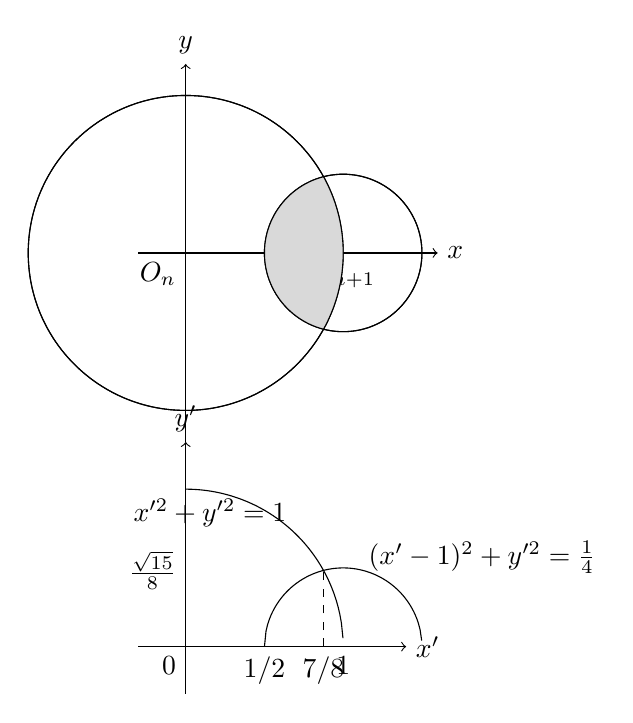
\begin{tikzpicture}[scale=2.0]
  \draw[->] (-0.3,0) -- (1.6,0) node[right] {$x$};
  \draw[->] (0,-1.2) -- (0,1.2) node[above] {$y$};
  \node[below left] at (0,0) {$O_n$};
  
  \draw (0,0) circle (1);
  \draw (1,0) circle (0.5);
  \node[below] at (1,0) {$O_{n+1}$};
  \node[below right] at (0.5,0) {$\frac{a}{2^n}$};
  
  \begin{scope}
    \clip (0,0) circle (1);
    \clip (1,0) circle (0.5);
    \fill[gray!30] (-1,-1) rectangle (2,1);
  \end{scope}
  \draw (0,0) circle (1);
  \draw (1,0) circle (0.5);
  
  \begin{scope}[shift={(0,-2.5)}]
    \draw[->] (-0.3,0) -- (1.4,0) node[right] {$x'$};
    \draw[->] (0,-0.3) -- (0,1.3) node[above] {$y'$};
    \node[below left] at (0,0) {$0$};
    
    \draw[domain=0:1,samples=100] plot (\x, {sqrt(1-\x*\x)});
    \draw[domain=0.5:1.5,samples=100] plot (\x, {sqrt(0.25-(\x-1)*(\x-1))});
    
    \node[above left] at (0.7,0.7) {$x'^2+y'^2=1$};
    \node[above right] at (1.1,0.4) {$(x'-1)^2+y'^2=\frac{1}{4}$};
    
    \draw[dashed] (7/8,0) -- (7/8, {sqrt(1-49/64)});
    \node[below] at (7/8,0) {$7/8$};
    \node[below] at (1/2,0) {$1/2$};
    \node[below] at (1,0) {$1$};
    \node[left] at (0, {sqrt(15)/8}) {$\frac{\sqrt{15}}{8}$};
  \end{scope}
\end{tikzpicture}
\caption{球 $S_n, S_{n+1}$ の断面円 $C_n, C_{n+1}$ の交点}
\end{figure}

\end{document}
